\documentclass[titlepage, 12pt]{article}

\usepackage[margin=1in]{geometry}
\usepackage[hidelinks]{hyperref}
\usepackage{amsmath}
\usepackage{float}
\usepackage{graphicx}
% \usepackage{newtxtext}  % WHY IS THIS HERE
\usepackage{listings}
\usepackage{circuitikz}
\usepackage{color}
\usepackage{multicol}

% Default fixed font does not support bold face
\DeclareFixedFont{\ttb}{T1}{txtt}{bx}{n}{10} % for bold
\DeclareFixedFont{\ttm}{T1}{txtt}{m}{n}{10}

% Define colors
\definecolor{deepblue}{rgb}{0,0,0.5}
\definecolor{deepred}{rgb}{0.6,0,0}
\definecolor{deepgreen}{rgb}{0,0.5,0}


% Python style for highlighting
\newcommand\pythonstyle{\lstset{
    language=Python,
    basicstyle=\ttm,
    otherkeywords={self},             % Add keywords here
    keywordstyle=\ttb\color{deepblue},
    emph={bin,_prod,__name__},          % Custom highlighting
    emphstyle=\ttb\color{deepred},    % Custom highlighting style
    stringstyle=\color{deepgreen},
    commentstyle=\color{deepgreen},
    frame=tb,
    % Any extra options here
    showstringspaces=false
}}
\newcommand\pythonexternal[2][]{{\pythonstyle\lstinputlisting[#1]{#2}}}
\newcommand\bbar[1]{\mathop{\overline{#1 \vphantom A}}}
\newcommand\sA{\ensuremath{\mathtt{A}}}
\newcommand\sB{\ensuremath{\mathtt{B}}}

% Author information
\title{ENCM 467 Lab 3\\Static and Dynamic Behaviour of CMOS logic Gates}
\author{Andreas Smit}
\date{November 20, 2020}

% Settings
\setlength{\parindent}{0pt}

\begin{document}
    \maketitle

    \section{CMOS Digital Logic Gates}\label{sec:gates}
    There are 2 digital logic gates that will be used throughout this
    lab, a CMOS NAND gate (figure \ref{fig:NAND}) and CMOS NOR gate
    (figure \ref{fig:NOR}).
    \begin{multicols}{2}
        \begin{figure}[H]
            \centering
            \begin{circuitikz}
                \draw (-1, 5) node[pmos](QPA){}
                (QPA.G)node[left]{$\mathtt{A}$};
                \draw (1, 5) node[pmos, xscale=-1](QPB){}
                (QPB.G)node[right]{$\mathtt{B}$};
                \draw (0, 3) node[nmos](QNB){}
                (QNB.G)node[left]{$\mathtt{B}$};
                \draw (0, 1) node[nmos](QNA){}
                (QNA.G)node[left]{$\mathtt{A}$};
                \draw (QPA.S) node[vcc]{$V_{DD}$} (QPB.S)
                node[vcc]{$V_{DD}$};
                \draw (QPA.D) to (-1, 4) to (1, 4) to (QPB.D) (1, 4) to
                (1.5, 4) node[right]{$V_{out} = \bbar{\sA\sB}$};
                \draw (0, 4) to (QNB.D);
                \draw (QNB.S) to (QNA.D);
                \draw (QNA.S) node[vee]{$V_{SS}$};
            \end{circuitikz}
            \caption{A CMOS NAND Gate}
            \label{fig:NAND}
        \end{figure}
        \begin{figure}[H]
            \centering
            \begin{circuitikz}
                \draw (0, 5) node[pmos](QPA){}
                (QPA.G)node[left]{$\mathtt{A}$};
                \draw (0, 3) node[pmos](QPB){}
                (QPB.G)node[left]{$\mathtt{B}$};
                \draw (1, 1) node[nmos, xscale=-1](QNB){}
                (QNB.G)node[right]{$\mathtt{B}$};
                \draw (-1, 1) node[nmos](QNA){}
                (QNA.G)node[left]{$\mathtt{A}$};
                \draw (QPA.S) node[vcc]{$V_{DD}$};
                \draw (QPA.D) to (QPB.S);
                \draw (QPB.D) to (0, 2) (QNA.D) to (-1, 2) to (1, 2) to
                (QNB.D) (1, 2) to (1.5, 2)
                node[right]{$V_{out} = \bbar{\sA + \sB}$};
                \draw (QNA.S) node[vee]{$V_{SS}$} (QNB.S)
                node[vee]{$V_{SS}$};
            \end{circuitikz}
            \caption{A CMOS NOR Gate}
            \label{fig:NOR}
        \end{figure}
    \end{multicols}
    The NAND and NOR gates are implemented in LTspice using the CD 4007
    CMOS integrated circuit as shown in figures \ref{fig:NAND_lt} and
    \ref{fig:NOR_lt} respectively. All inputs not used are tied to
    ground to prevent floating inputs.
    \begin{multicols}{2}
        \begin{figure}[H]
            \centering
            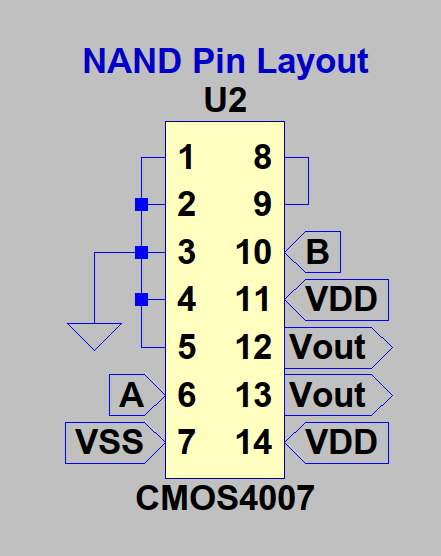
\includegraphics[width=0.4\linewidth]{figures/NAND_circuit.png}
            \caption{The NAND circuit built in LTspice.}
            \label{fig:NAND_lt}
        \end{figure}
        \begin{figure}[H]
            \centering
            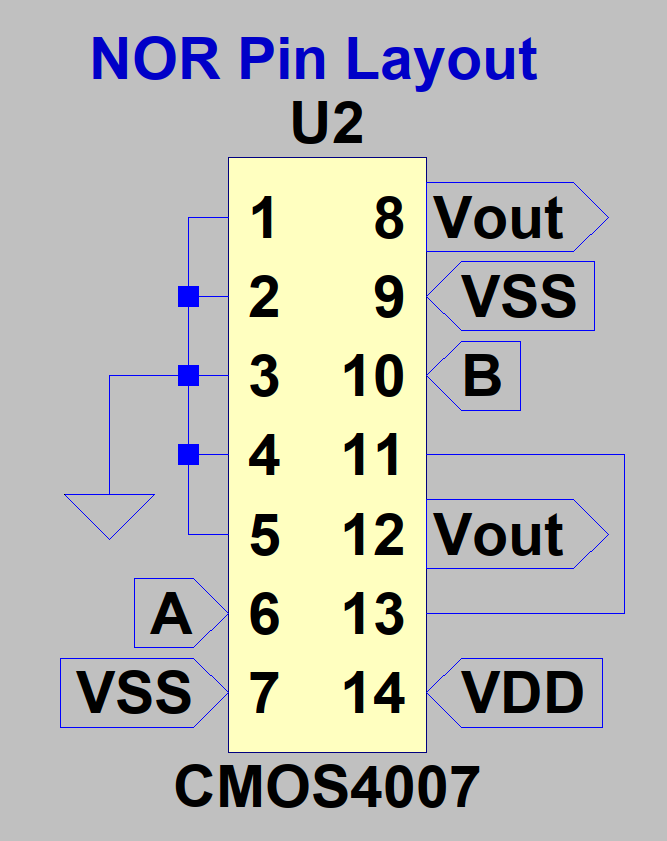
\includegraphics[width=0.4\linewidth]{figures/NOR_circuit.png}
            \caption{The NOR circuit built in LTspice.}
            \label{fig:NOR_lt}
        \end{figure}
    \end{multicols}
    The NAND and NOR circuits are then exported as a sub circuit similar
    to the CMOS4007 component so that they can be reused throughout the
    rest of the lab as a discrete component.

    \section{Logic Gate Measurements}
    \subsection{Static Behaviour of CMOS NAND and NOR Gates}
    \subsubsection{NAND Gate Measurements}
    The static measurements of the CMOS NAND gate is done using the
    circuit setup in LTspice shown in figure \ref{fig:part_21_NAND}.
    Note that the NAND gate use (as with all NAND gates in the lab) is
    the NAND gate as designed in section \ref{sec:gates}.
    \begin{figure}[H]
        \centering
        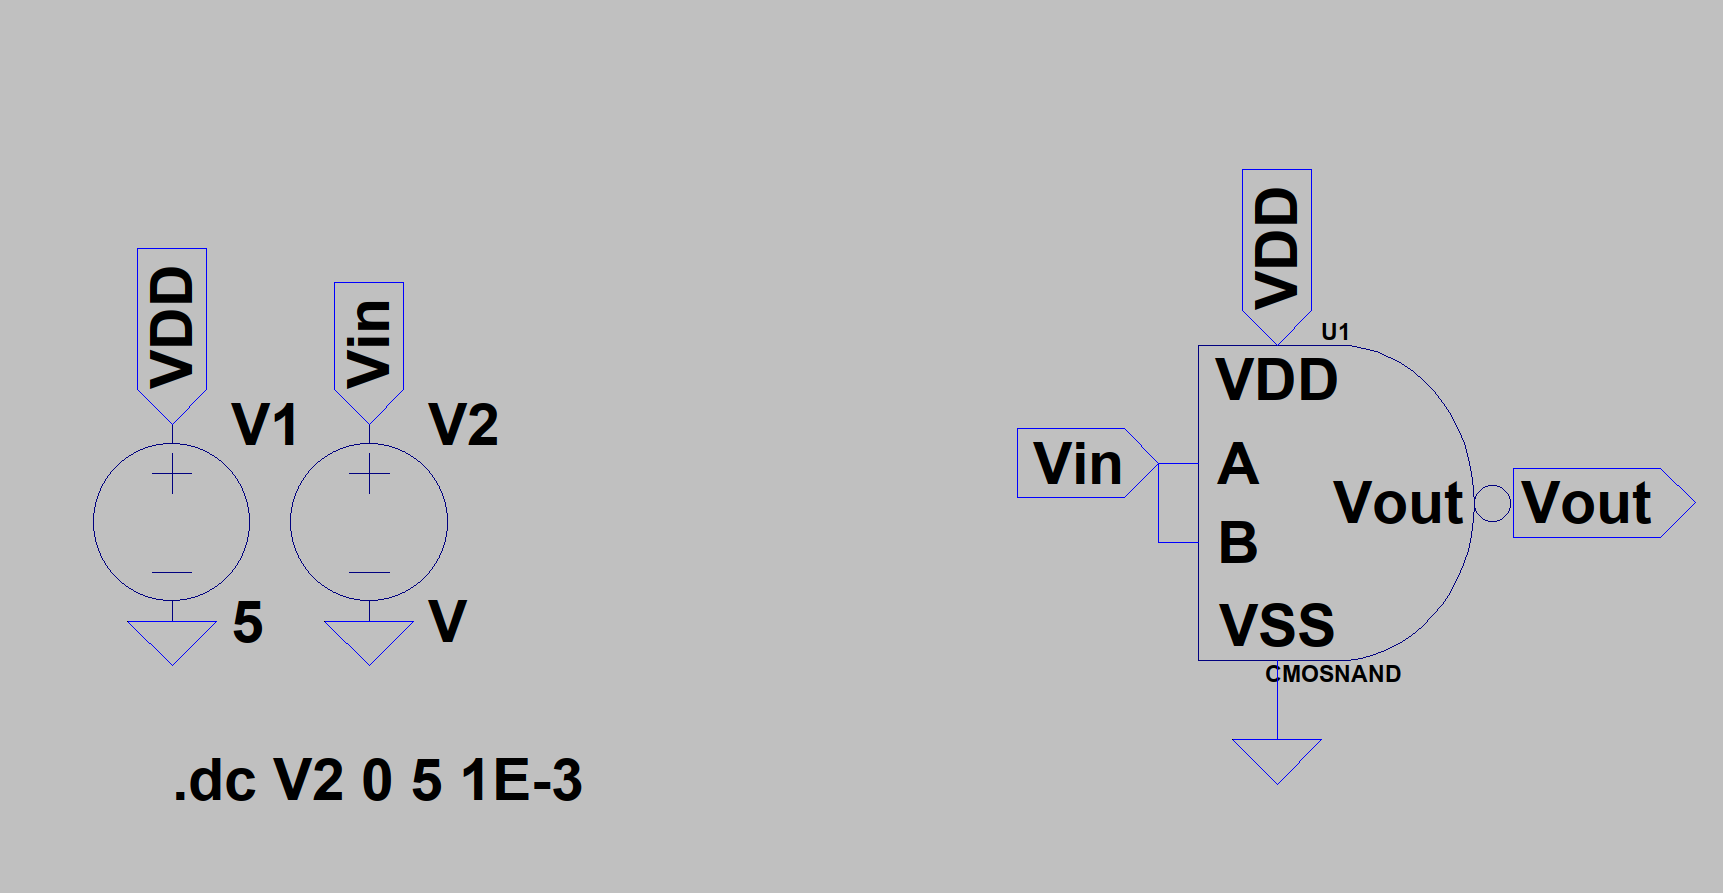
\includegraphics[width=0.6\textwidth]{figures/part_21_NAND_circuit.png}
        \caption{The NAND gate circuit in LTspice for measuring the
        static properties of the NAND gate.}
        \label{fig:part_21_NAND}
    \end{figure}
    When the DC analysis is run on the circuit above the voltage
    transfer curve in figure \ref{fig:NAND_VTC} is generated.
    \begin{figure}[H]
        \centering
        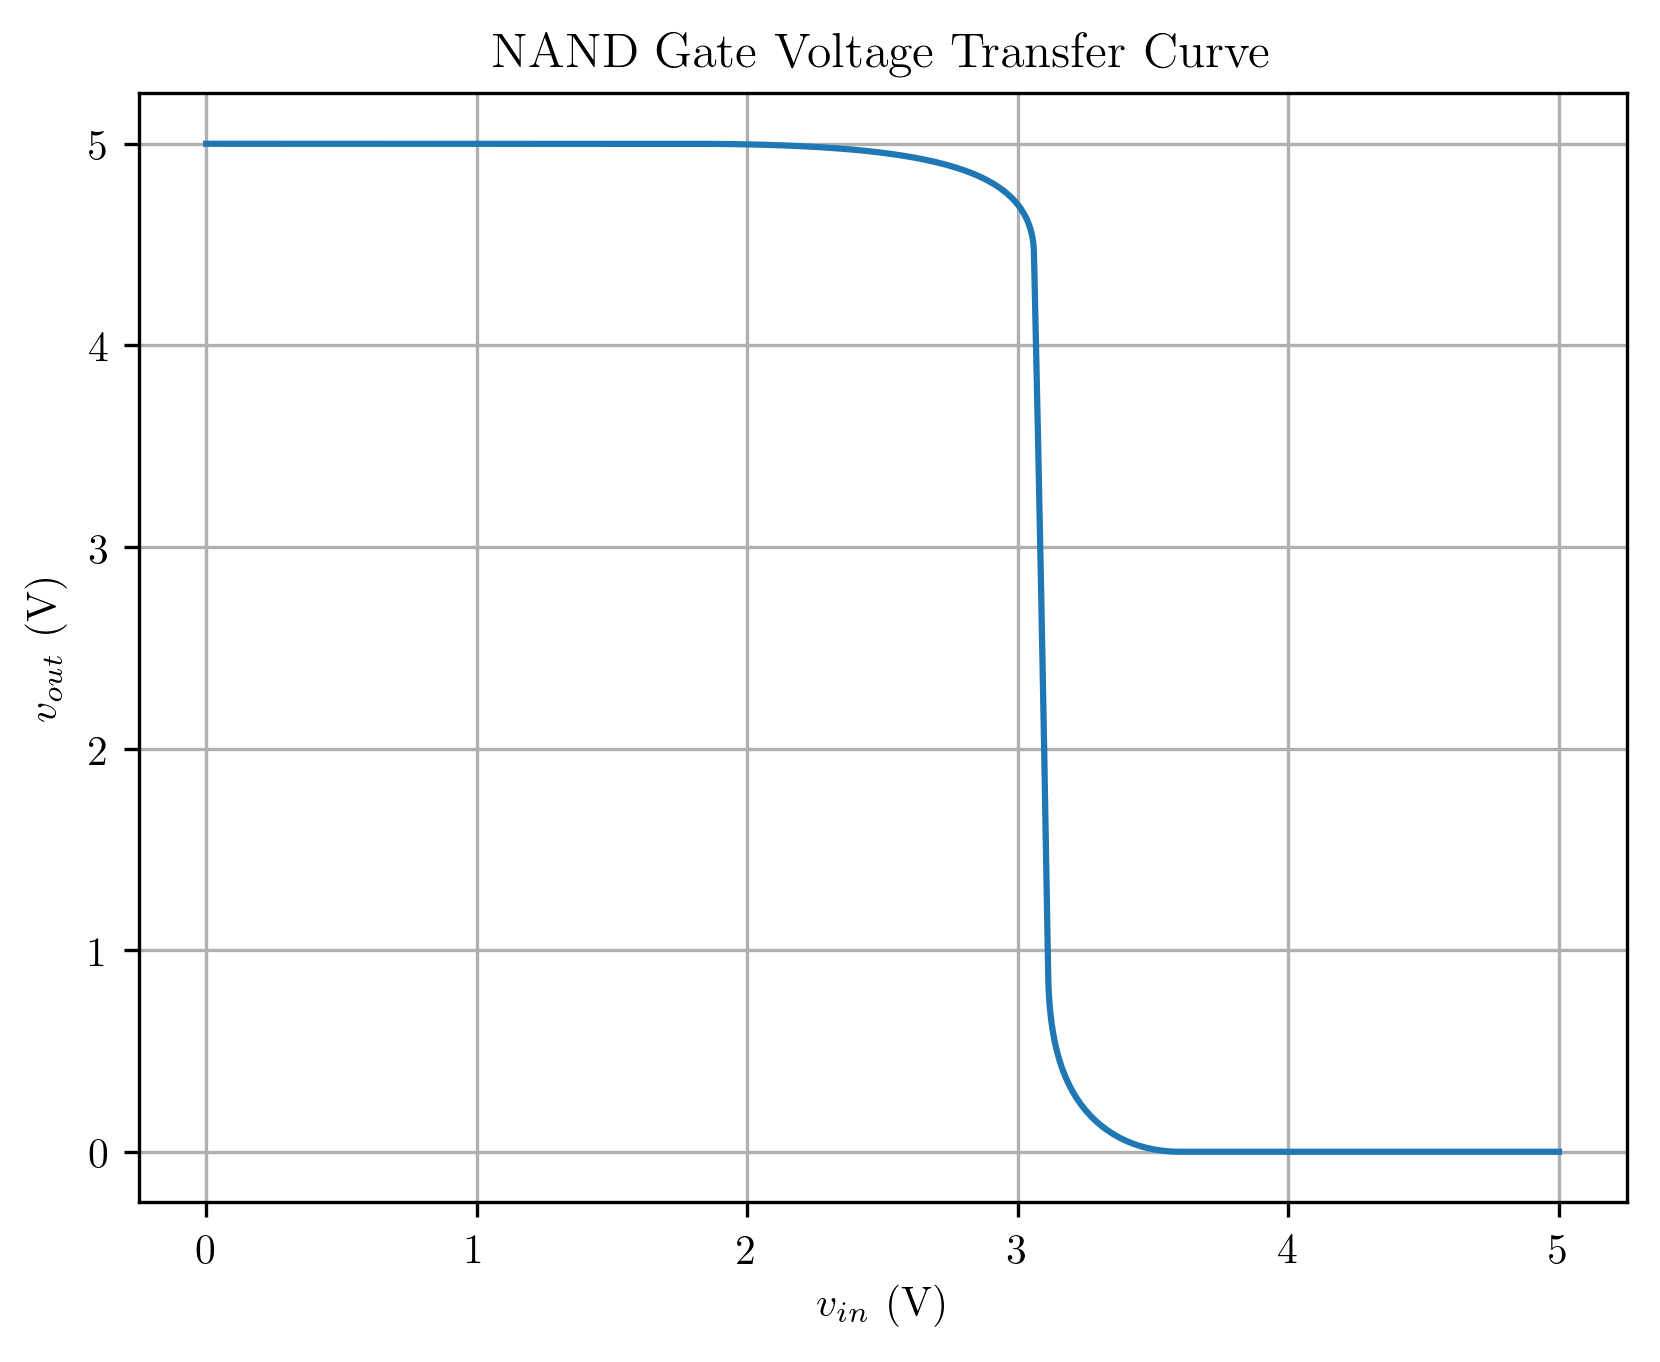
\includegraphics[width=0.6\textwidth]{figures/part_21_NAND.png}
        \caption{The Voltage transfer characteristics for the CMOS NAND
        gate.}
        \label{fig:NAND_VTC}
    \end{figure}
    Then the python code in appendix \ref{sec:code} is used to caluclate
    the critical voltage values which are given in table
    \ref{tab:NAND_volt}.
    \begin{table}[H]
        \centering
        \caption{The critical voltages for the CMOS NAND gate.}
        \label{tab:NAND_volt}
        \begin{tabular}{c|c}
            & Voltage (V)\\
            \hline
            $V_{IL}$ & 2.942\\
            $V_{IH}$ & 3.321\\
            $V_{OH}$ & 5\\
            $V_{OL}$ & 0\\
            $V_{INV}$ & 3.055\\
            $NM_L$ & 2.942\\
            $NM_H$ & 1.679\\
        \end{tabular}
    \end{table}
    \subsubsection{NOR Gate Measurements}
    The static measurements of the CMOS NOR gate is done using the
    circuit setup in LTspice shown in figure \ref{fig:part_21_NOR}.
    Note that the NOR gate use (as with all NOR gates in the lab) is
    the NOR gate as designed in section \ref{sec:gates}.
    \begin{figure}[H]
        \centering
        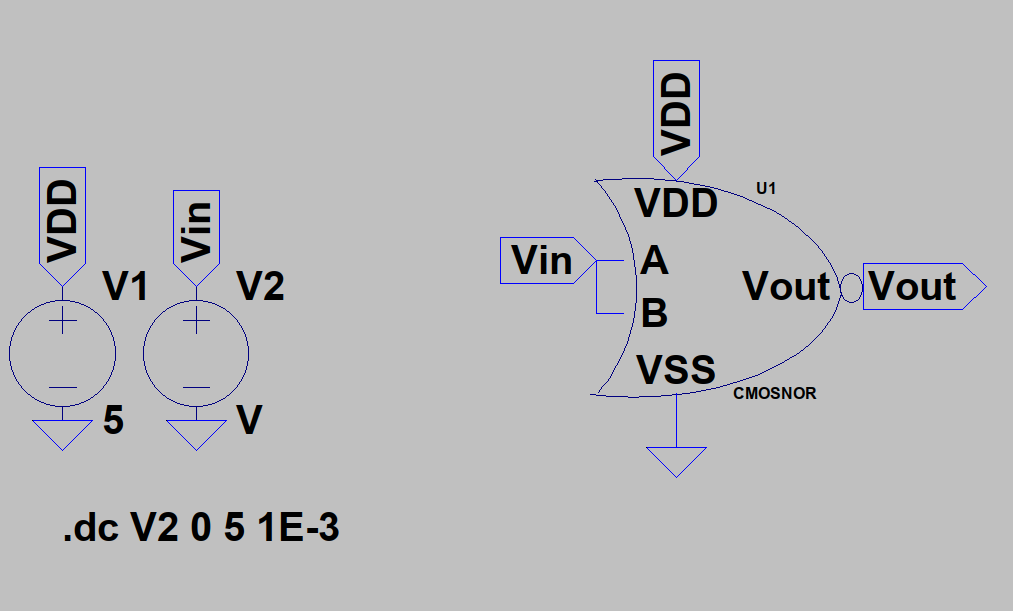
\includegraphics[width=0.6\textwidth]{figures/part_21_NOR_circuit.png}
        \caption{The NOR gate circuit in LTspice for measuring the
        static properties of the NOR gate.}
        \label{fig:part_21_NOR}
    \end{figure}
    When the DC analysis is run on the circuit above the voltage
    transfer curve in figure \ref{fig:NOR_VTC} is generated.
    \begin{figure}[H]
        \centering
        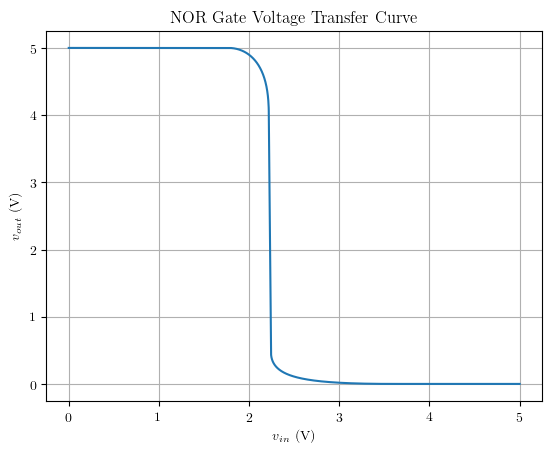
\includegraphics[width=0.6\textwidth]{figures/part_21_NOR.png}
        \caption{The Voltage transfer characteristics for the CMOS NOR
        gate.}
        \label{fig:NOR_VTC}
    \end{figure}
    Then the python code in appendix \ref{sec:code} is used to caluclate
    the critical voltage values which are given in table
    \ref{tab:NOR_volt}.
    \begin{table}[H]
        \centering
        \caption{The critical voltages for the CMOS NOR gate.}
        \label{tab:NOR_volt}
        \begin{tabular}{c|c}
            & Voltage (V)\\
            \hline
            $V_{IL}$ & 1.997\\
            $V_{IH}$ & 2.339\\
            $V_{OH}$ & 5\\
            $V_{OL}$ & 0\\
            $V_{INV}$ & 2.226\\
            $NM_L$ & 1.997\\
            $NM_H$ & 2.661\\
        \end{tabular}
    \end{table}

    \subsubsection{Static Gate Properties Analysis}
    Recall that for a CMOS inverter $V_{INV}$ is given by
    \begin{equation}\label{eq:inv}
        V_{INV} =
        \frac{V_{T0(n)} + \sqrt{\frac{k_p}{k_n}}(V_{DD} -|V_{T0(p)}|)}
        {1 + \sqrt{\frac{k_p}{k_n}}}
    \end{equation}
    From equation \eqref{eq:inv} we can see that the threshold voltage
    is related to
    $\left(\frac{W}{L}\right)_p\left(\frac{L}{W}\right)_n$. We know that
    for an ideal inverter $W_p = 2W_n$ which roughly corresponds to a
    $V_{INV} = \frac{V_{DD}}{2}$. If we assume the width of the
    PMOS transistors used in the circuit is twice that of the NMOS, then
    we would have a width ratio of $2\frac{2W}{L}$ for the PMOS and
    $\frac{W}{2L}$ for the NMOS in the NAND gate. This would
    scale $\frac{k_p}{k_n}$ by a factor of 4 which would increase the
    inversion voltage which is what we see in the NAND gate. Similarly
    for the NOR gate, if we assume the width of the PMOS transistor used
    in the circuit is twice that of the NMOS, then we would have a width
    ration of $\frac{W}{L}$ for the PMOS transistors and $\frac{2W}{L}$
    for the NMOS transistors. This would scale $\frac{k_p}{k_n}$ by a
    factor of $\frac{1}{4}$ decreasing the inversion voltage which is
    what we see for the NOR gate. As the other critical voltages are
    also related to $\frac{k_p}{k_n}$ a similar argument can be made.

    \pagebreak
    \subsection{Dynamic Behaviour of CMOS NAND and NOR gates}
    \subsubsection{NAND Gate Measurements}\label{sec:NAND_time}
    \paragraph{NAND Gate Measurements With Variable $\mathtt{A}$
    Input}

    The dynamic measurements of the CMOS NAND with the variable $\sA$ input
    is done using the circuit setup in LTspice shown in figure
    \ref{fig:part_22_NAND_A_circuit}.
    \begin{figure}[H]
        \centering
        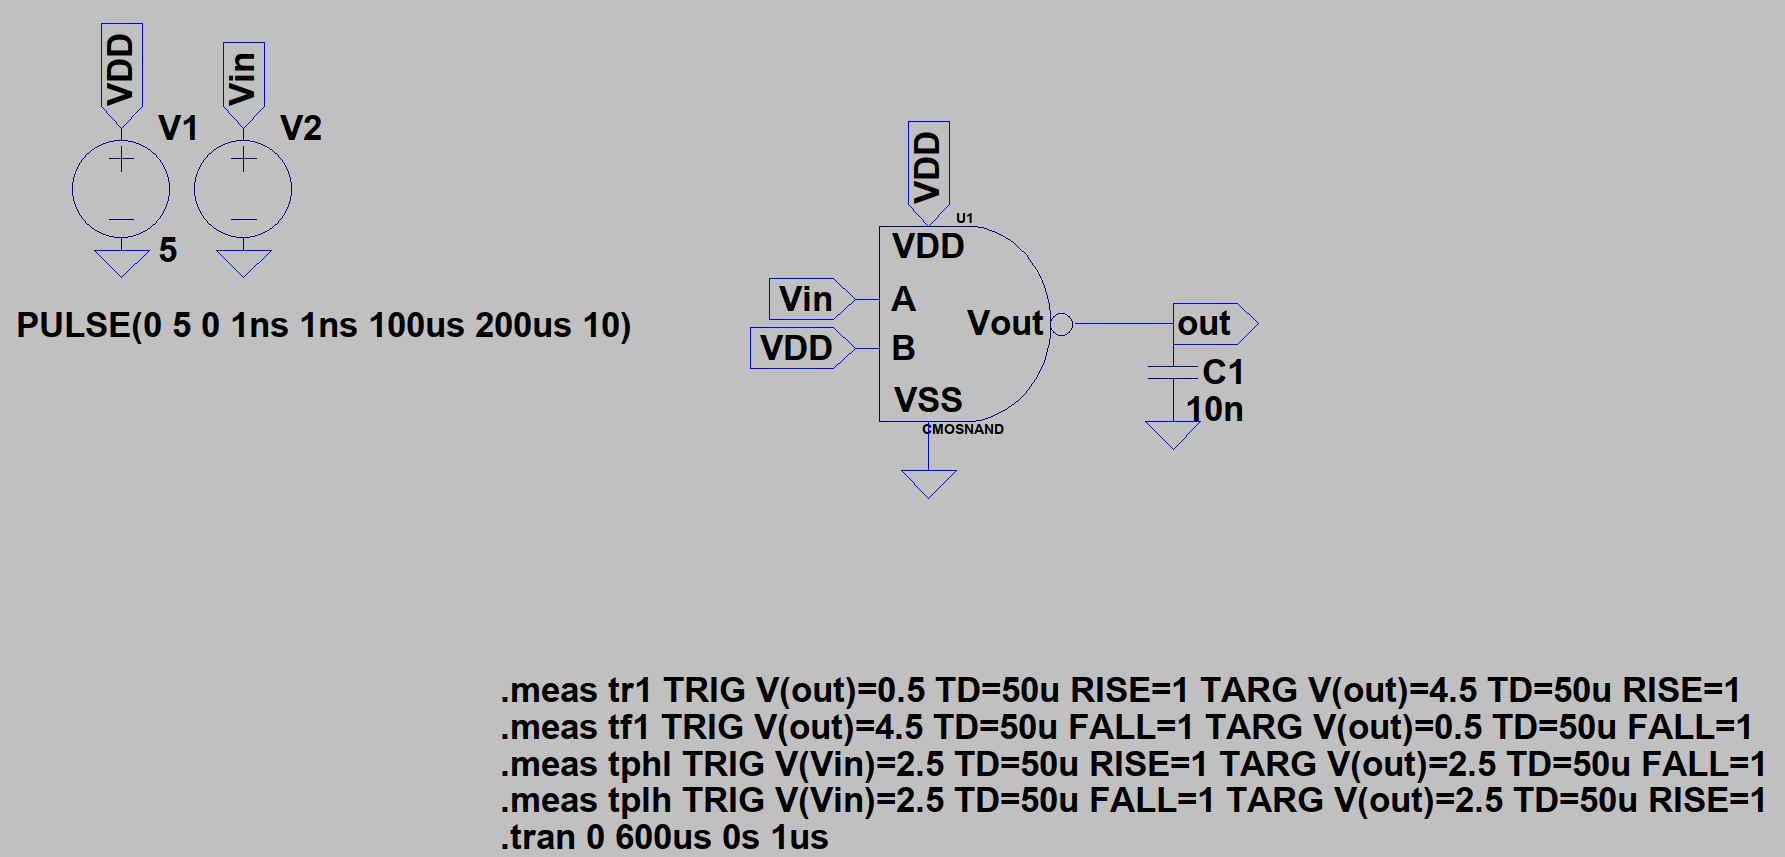
\includegraphics[width=0.6\textwidth]
        {figures/part_22_NAND_A_circuit.png}
        \caption{The NAND gate circuit in LTspice for measuring the
            dynamic properties of the NAND gate with $\sA$ as a variable
        input}
        \label{fig:part_22_NAND_A_circuit}
    \end{figure}
    When the transient analysis is run on the circuit above the response
    in figure \ref{fig:part_22_NAND_A} is generated.
    \begin{figure}[H]
        \centering
        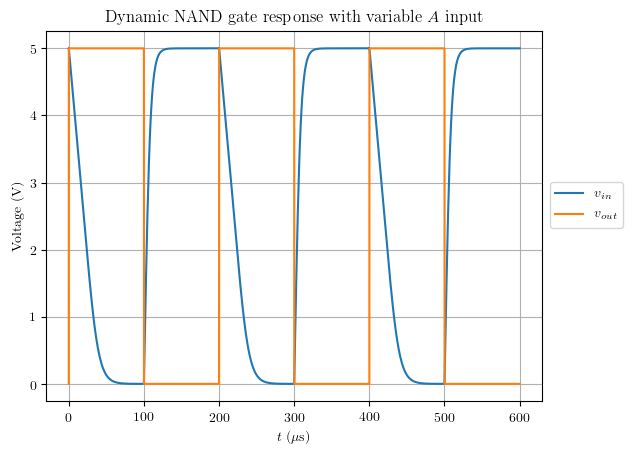
\includegraphics[width=0.6\textwidth]{figures/part_22_NAND_A.png}
        \caption{The transient response for the CMOS NAND gate with a
        variable $\sA$ input and constant $\sB$ input.}
        \label{fig:part_22_NAND_A}
    \end{figure}
    Then the measure statements in the circuit are used to determine the
    timing values given in table \ref{tab:NAND_A_time}.
    \begin{table}[H]
        \centering
        \caption{The timing values for the CMOS NAND gate with variable
        $\sA$ input.}
        \label{tab:NAND_A_time}
        \begin{tabular}{c|c}
            & $Time$ ($\mu$s)\\
            \hline
            $t_{rise}$ & 11.606\\
            $t_{fall}$ & 35.274\\
            $t_{PLH}$ & 4.685\\
            $t_{PHL}$ & 19.973\\
            $t_s$ & 12.329\\
        \end{tabular}
    \end{table}
    \paragraph{NAND Gate Measurements With Variable $\mathtt{B}$
    Input}

    The dynamic measurements of the CMOS NAND with the variable $\sB$ input
    is done using the circuit setup in LTspice shown in figure
    \ref{fig:part_22_NAND_B_circuit}.
    \begin{figure}[H]
        \centering
        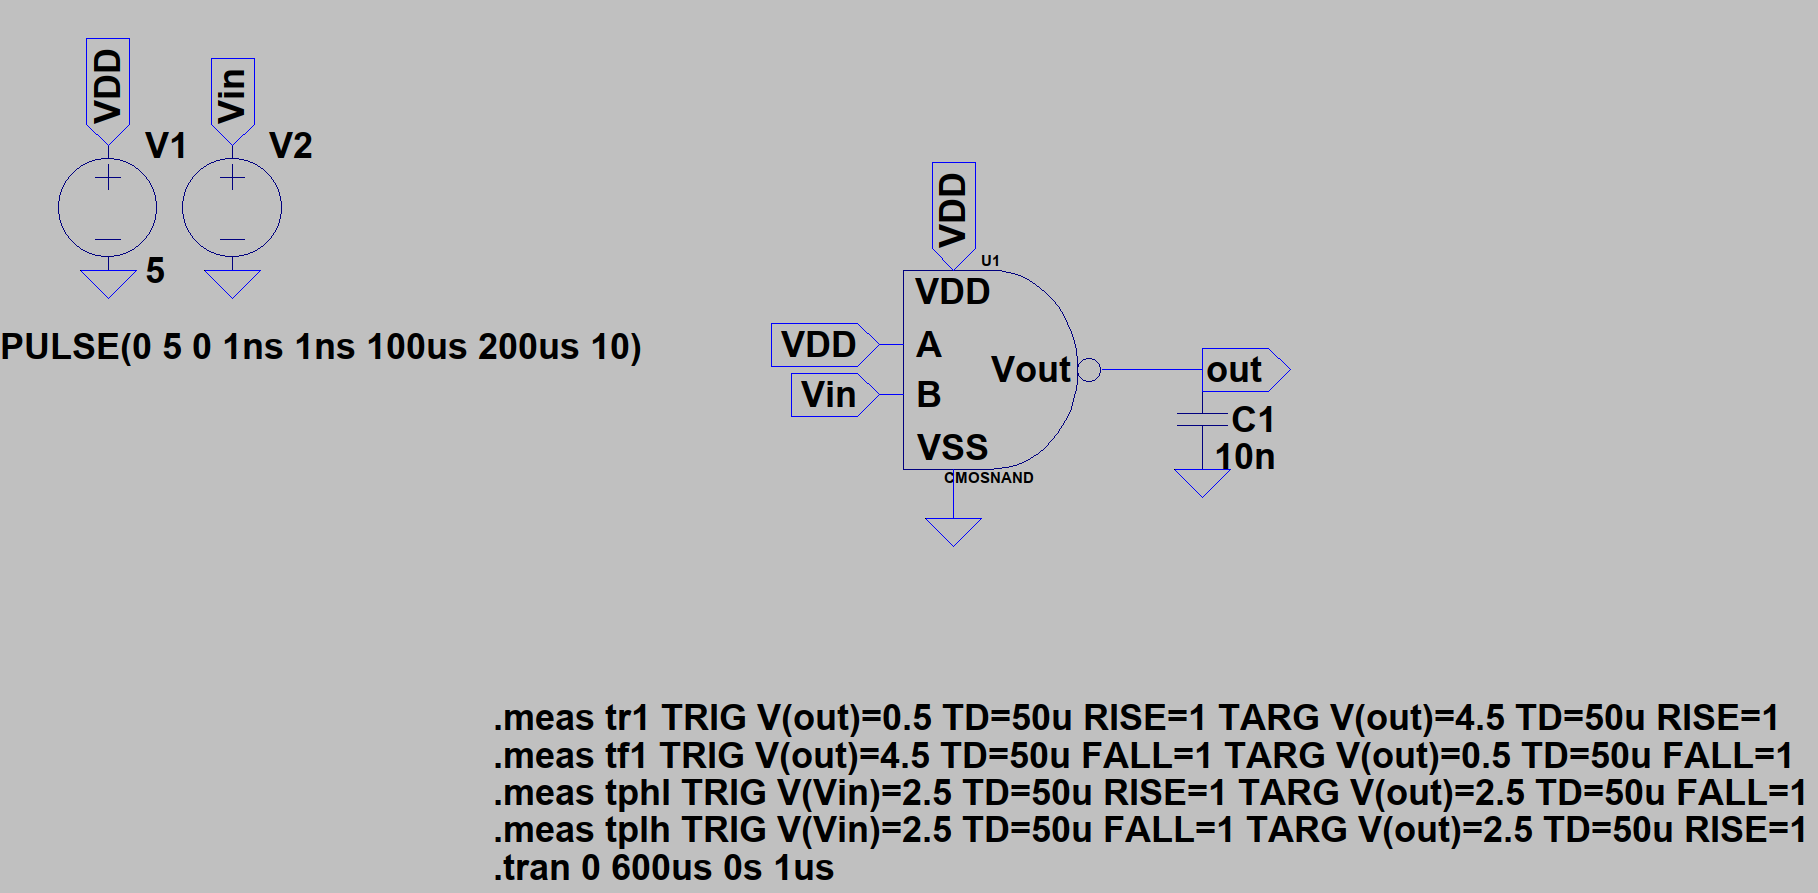
\includegraphics[width=0.6\textwidth]
        {figures/part_22_NAND_B_circuit.png}
        \caption{The NAND gate circuit in LTspice for measuring the
            dynamic properties of the NAND gate with $\sB$ as a variable
        input}
        \label{fig:part_22_NAND_B_circuit}
    \end{figure}
    When the transient analysis is run on the circuit above the response
    in figure \ref{fig:part_22_NAND_B} is generated.
    \begin{figure}[H]
        \centering
        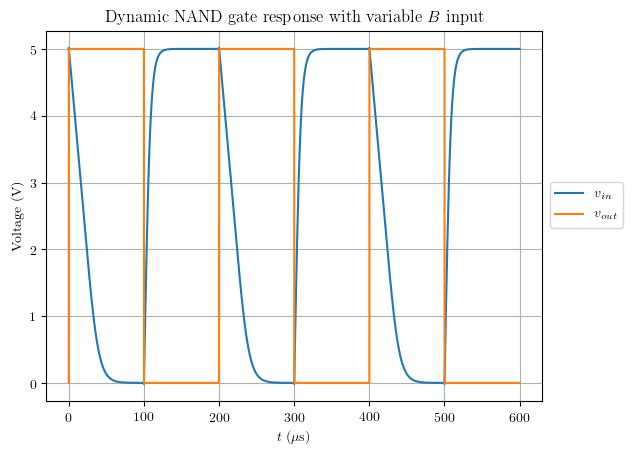
\includegraphics[width=0.6\textwidth]{figures/part_22_NAND_B.png}
        \caption{The transient response for the CMOS NAND gate with a
        variable $\sB$ input and constant $\sA$ input.}
        \label{fig:part_22_NAND_B}
    \end{figure}
    Then the measure statements in the circuit are used to determine the
    timing values given in table \ref{tab:NAND_B_time}.
    \begin{table}[H]
        \centering
        \caption{The timing values for the CMOS NAND gate with variable
        $\sB$ input.}
        \label{tab:NAND_B_time}
        \begin{tabular}{c|c}
            & $Time$ ($\mu$s)\\
            \hline
            $t_{rise}$ & 11.594\\
            $t_{fall}$ & 35.268\\
            $t_{PLH}$ & 4.703\\
            $t_{PHL}$ & 20.006\\
            $t_s$ & 12.355\\
        \end{tabular}
    \end{table}
    \paragraph{NAND Gate Measurements With Common Variable Inputs}

    The dynamic measurements of the CMOS NAND with the connected
    variable inputs is done using the circuit setup in LTspice shown
    in figure \ref{fig:part_22_NAND_AB_circuit}.
    \begin{figure}[H]
        \centering
        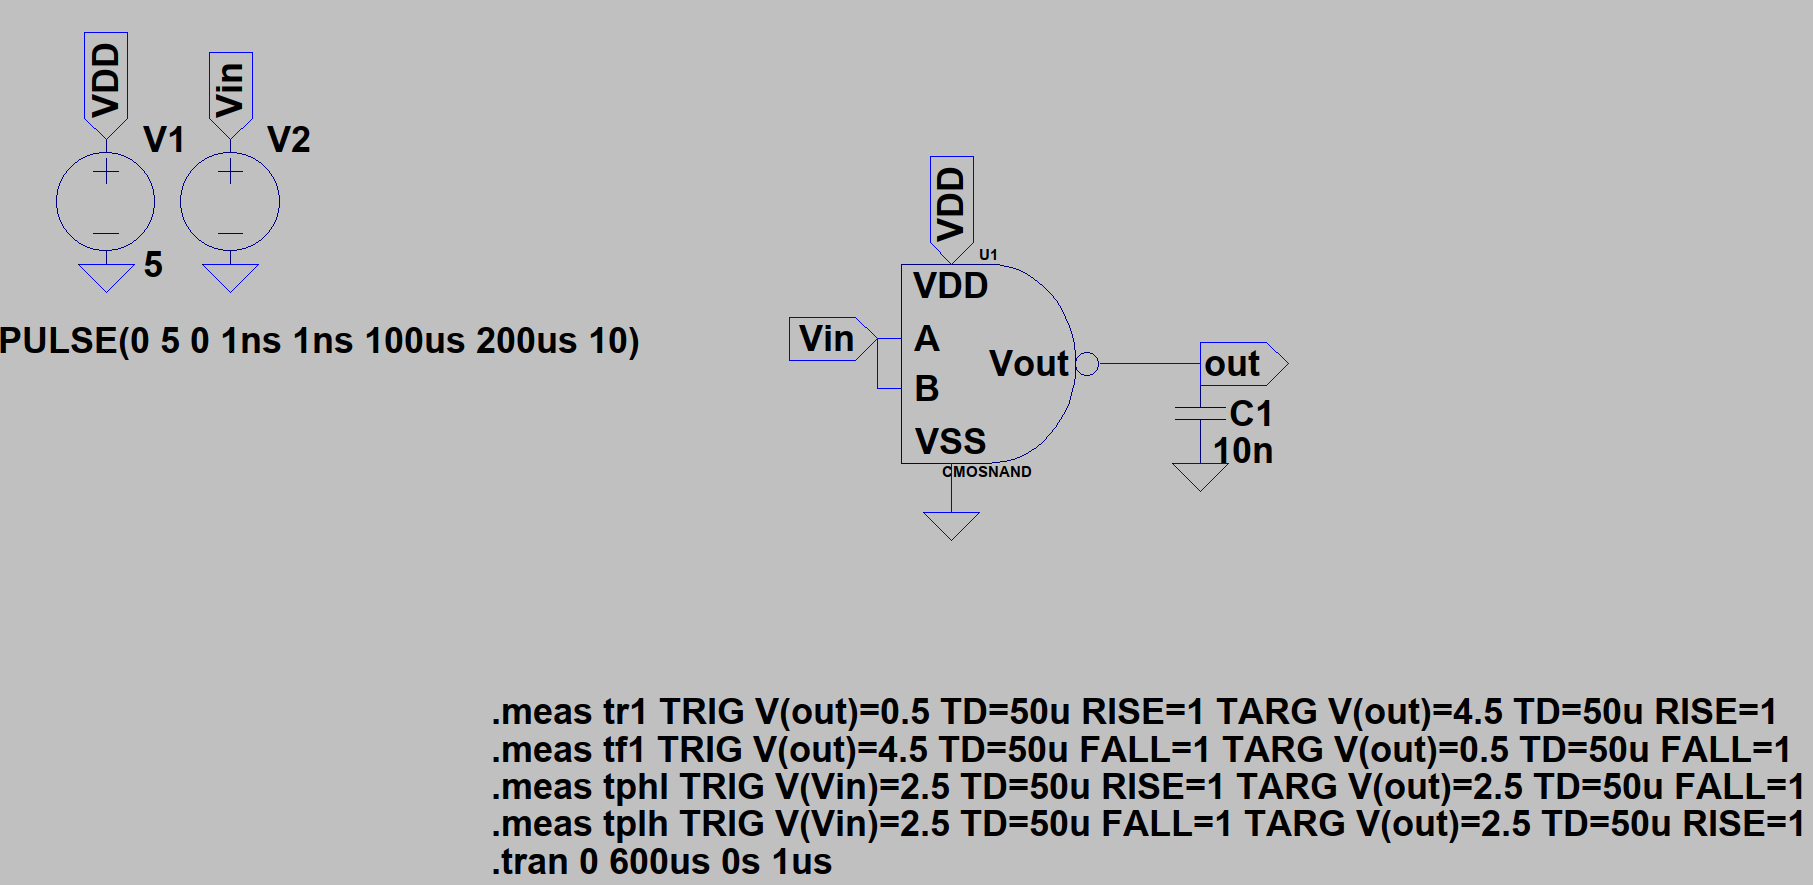
\includegraphics[width=0.6\textwidth]
        {figures/part_22_NAND_AB_circuit.png}
        \caption{The NAND gate circuit in LTspice for measuring the
            dynamic properties of the NAND gate with a common variable
        input}
        \label{fig:part_22_NAND_AB_circuit}
    \end{figure}
    When the transient analysis is run on the circuit above the response
    in figure \ref{fig:part_22_NAND_AB} is generated.
    \begin{figure}[H]
        \centering
        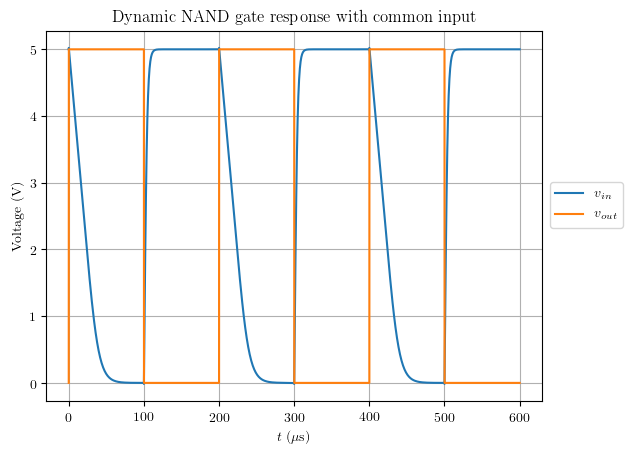
\includegraphics[width=0.6\textwidth]{figures/part_22_NAND_AB.png}
        \caption{The transient response for the CMOS NAND gate with a
        common variable input.}
        \label{fig:part_22_NAND_AB}
    \end{figure}
    Then the measure statements in the circuit are used to determine the
    timing values given in table \ref{tab:NAND_AB_time}.
    \begin{table}[H]
        \centering
        \caption{The timing values for the CMOS NAND gate with common
        variable inputs.}
        \label{tab:NAND_AB_time}
        \begin{tabular}{c|c}
            & $Time$ ($\mu$s)\\
            \hline
            $t_{rise}$ & 5.895\\
            $t_{fall}$ & 35.275\\
            $t_{PLH}$ & 2.411\\
            $t_{PHL}$ & 20.087\\
            $t_s$ & 11.249\\
        \end{tabular}
    \end{table}

    \pagebreak
    \subsubsection{NOR Gate Measurements}
    \paragraph{NOR Gate Measurements With Variable $\mathtt{A}$
    Input}

    The dynamic measurements of the CMOS NOR with the variable $\sA$ input
    is done using the circuit setup in LTspice shown in figure
    \ref{fig:part_22_NOR_A_circuit}.
    \begin{figure}[H]
        \centering
        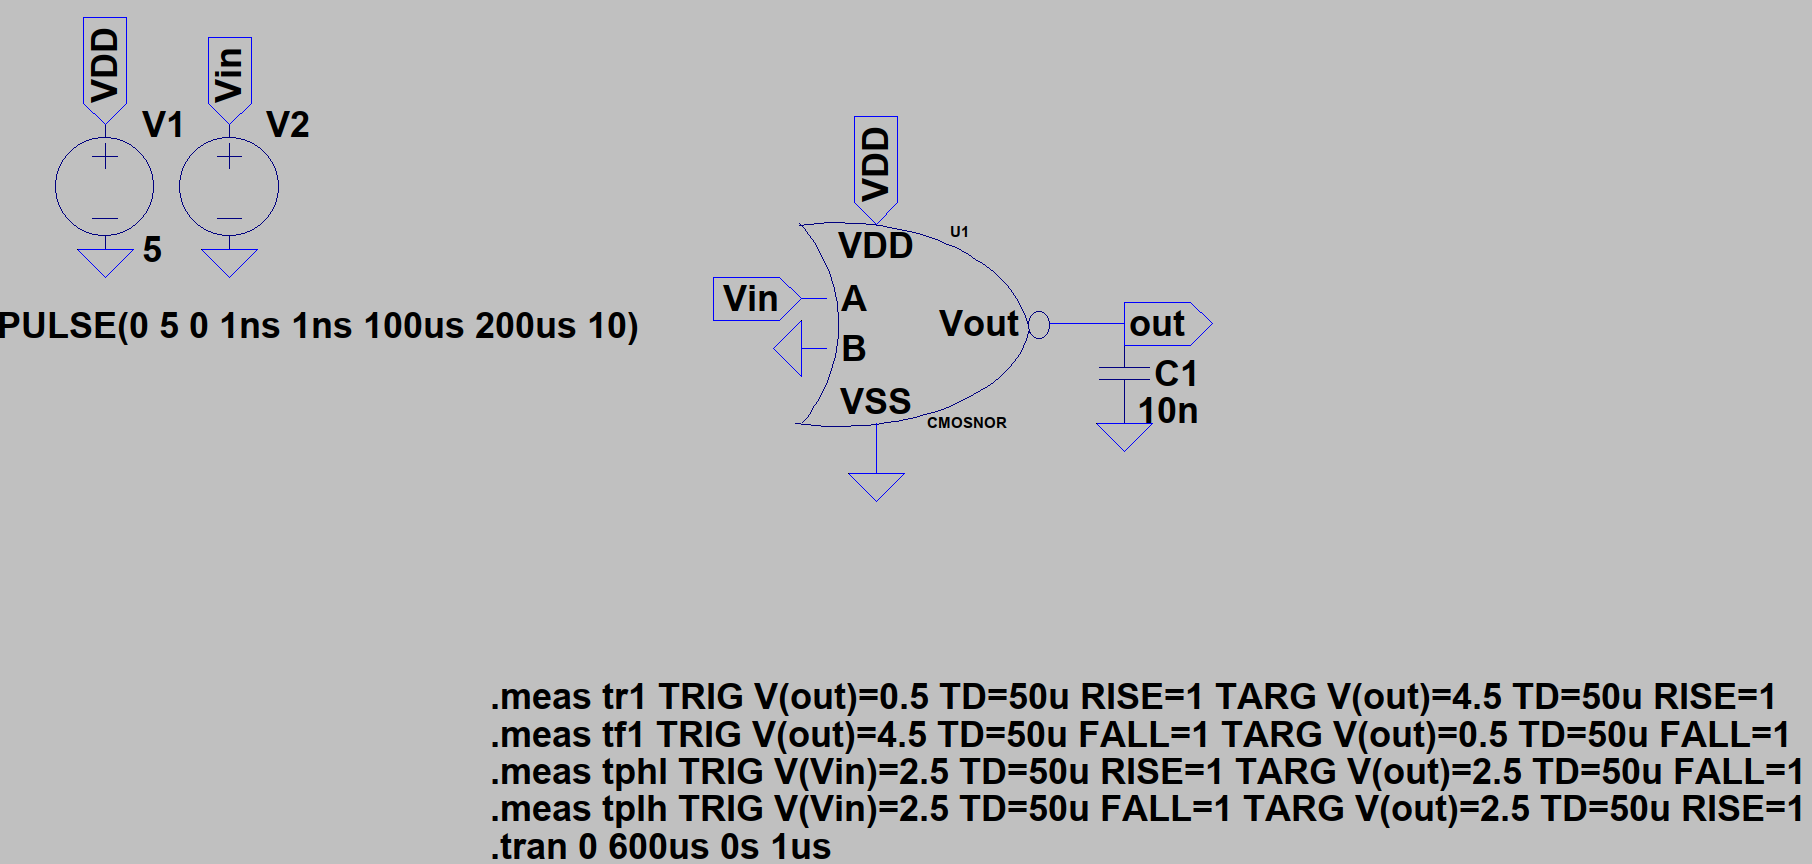
\includegraphics[width=0.6\textwidth]
        {figures/part_22_NOR_A_circuit.png}
        \caption{The NOR gate circuit in LTspice for measuring the
            dynamic properties of the NOR gate with $\sA$ as a variable
        input}
        \label{fig:part_22_NOR_A_circuit}
    \end{figure}
    When the transient analysis is run on the circuit above the response
    in figure \ref{fig:part_22_NOR_A} is generated.
    \begin{figure}[H]
        \centering
        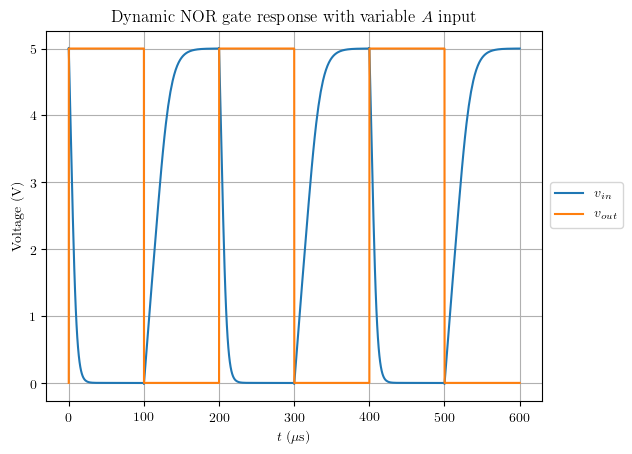
\includegraphics[width=0.6\textwidth]{figures/part_22_NOR_A.png}
        \caption{The transient response for the CMOS NOR gate with a
        variable $\sA$ input and constant $\sB$ input.}
        \label{fig:part_22_NOR_A}
    \end{figure}
    Then the measure statements in the circuit are used to determine the
    timing values given in table \ref{tab:NOR_A_time}.
    \begin{table}[H]
        \centering
        \caption{The timing values for the CMOS NOR gate with variable
        $\sA$ input.}
        \label{tab:NOR_A_time}
        \begin{tabular}{c|c}
            & $Time$ ($\mu$s)\\
            \hline
            $t_{rise}$ & 34.327\\
            $t_{fall}$ & 11.515\\
            $t_{PLH}$ & 17.868\\
            $t_{PHL}$ & 5.390\\
            $t_s$ & 11.629\\
        \end{tabular}
    \end{table}
    \paragraph{NOR Gate Measurements With Variable $\mathtt{B}$
    Input}

    The dynamic measurements of the CMOS NOR with the variable $\sB$ input
    is done using the circuit setup in LTspice shown in figure
    \ref{fig:part_22_NOR_B_circuit}.
    \begin{figure}[H]
        \centering
        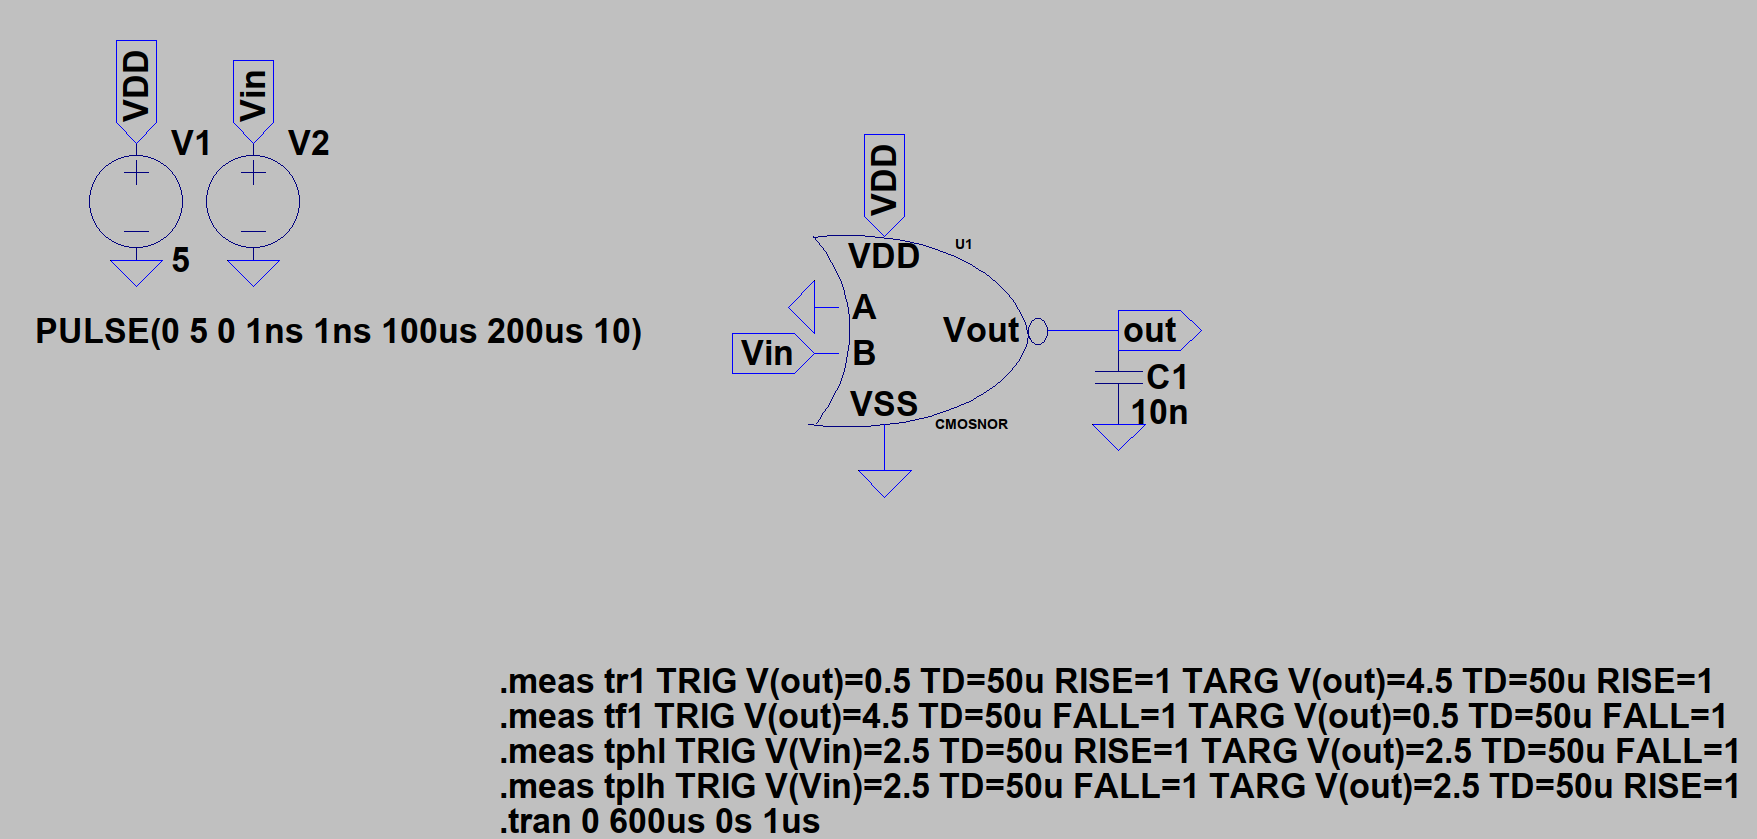
\includegraphics[width=0.6\textwidth]
        {figures/part_22_NOR_B_circuit.png}
        \caption{The NOR gate circuit in LTspice for measuring the
            dynamic properties of the NOR gate with $\sB$ as a variable
        input}
        \label{fig:part_22_NOR_B_circuit}
    \end{figure}
    When the transient analysis is run on the circuit above the response
    in figure \ref{fig:part_22_NOR_B} is generated.
    \begin{figure}[H]
        \centering
        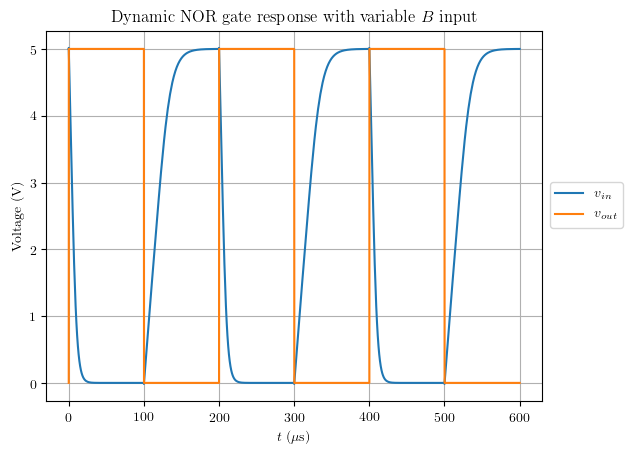
\includegraphics[width=0.6\textwidth]{figures/part_22_NOR_B.png}
        \caption{The transient response for the CMOS NOR gate with a
        variable $\sB$ input and constant $\sA$ input.}
        \label{fig:part_22_NOR_B}
    \end{figure}
    Then the measure statements in the circuit are used to determine the
    timing values given in table \ref{tab:NOR_B_time}.
    \begin{table}[H]
        \centering
        \caption{The timing values for the CMOS NOR gate with variable
        $\sB$ input.}
        \label{tab:NOR_B_time}
        \begin{tabular}{c|c}
            & $Time$ ($\mu$s)\\
            \hline
            $t_{rise}$ & 34.318\\
            $t_{fall}$ & 11.498\\
            $t_{PLH}$ & 17.837\\
            $t_{PHL}$ & 5.372\\
            $t_s$ & 11.605\\
        \end{tabular}
    \end{table}
    \paragraph{NOR Gate Measurements With Common Variable Inputs}

    The dynamic measurements of the CMOS NOR with the connected
    variable inputs is done using the circuit setup in LTspice shown
    in figure \ref{fig:part_22_NOR_AB_circuit}.
    \begin{figure}[H]
        \centering
        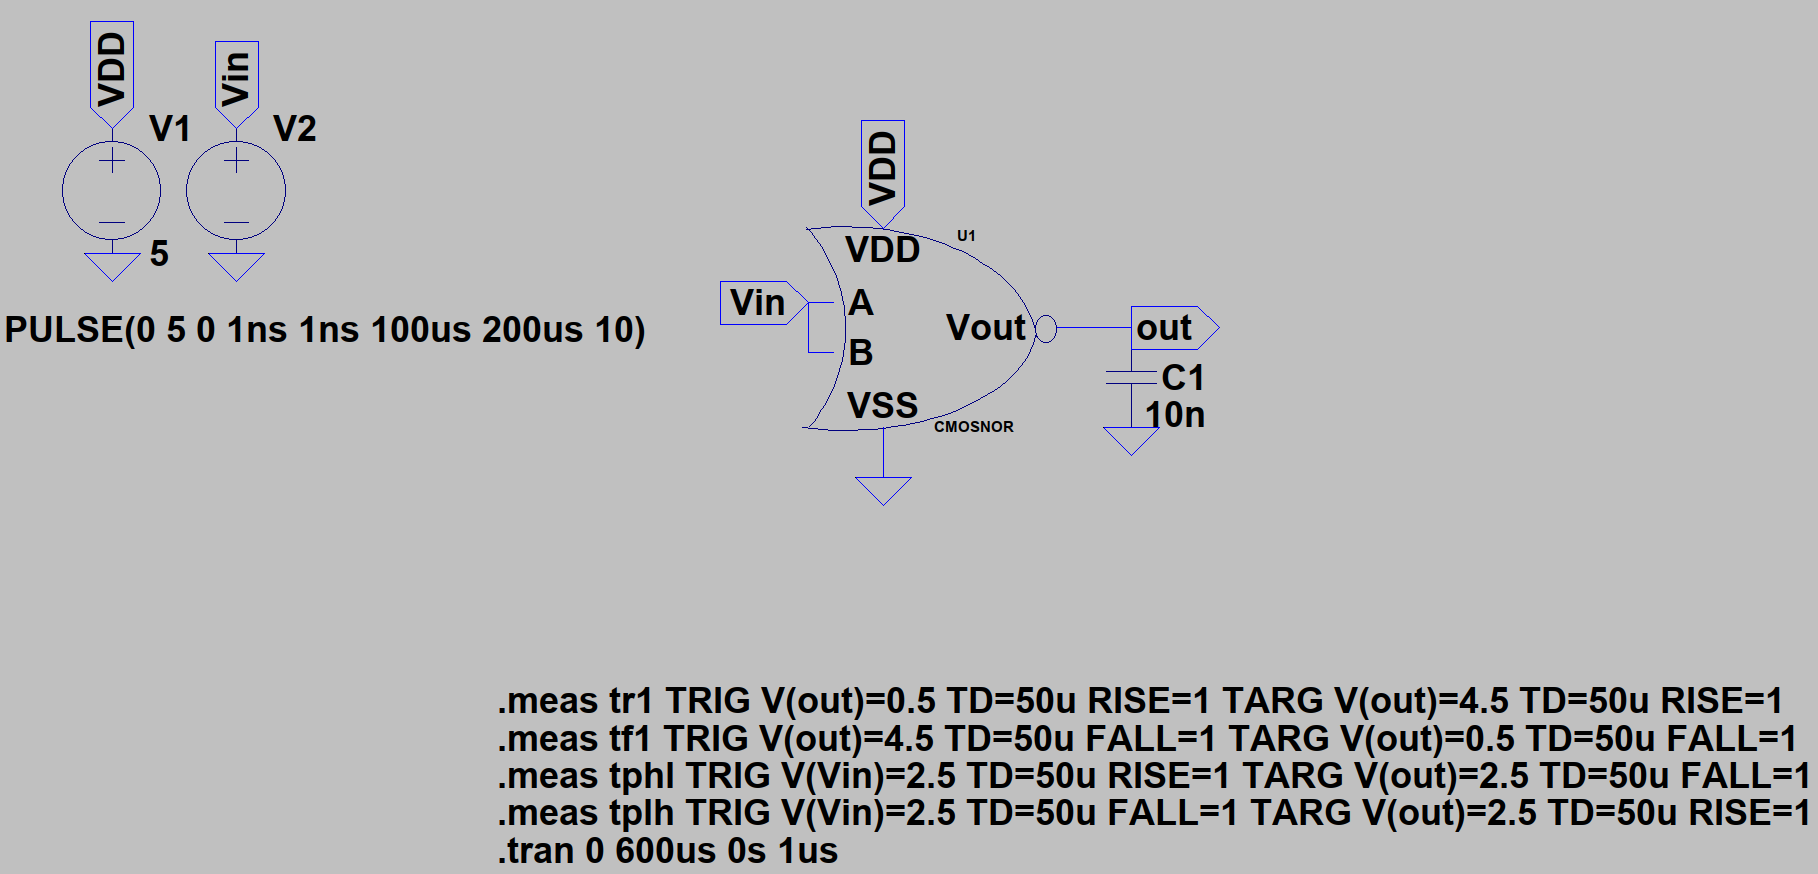
\includegraphics[width=0.6\textwidth]
        {figures/part_22_NOR_AB_circuit.png}
        \caption{The NOR gate circuit in LTspice for measuring the
            dynamic properties of the NOR gate with a common variable
        input}
        \label{fig:part_22_NOR_AB_circuit}
    \end{figure}
    When the transient analysis is run on the circuit above the response
    in figure \ref{fig:part_22_NOR_AB} is generated.
    \begin{figure}[H]
        \centering
        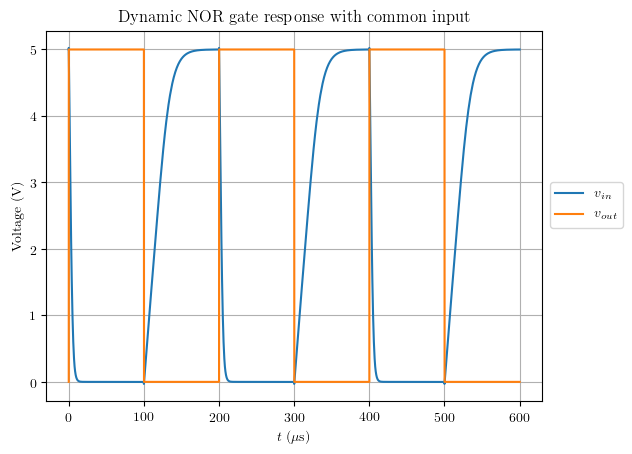
\includegraphics[width=0.6\textwidth]{figures/part_22_NOR_AB.png}
        \caption{The transient response for the CMOS NOR gate with a
        common variable input.}
        \label{fig:part_22_NOR_AB}
    \end{figure}
    Then the measure statements in the circuit are used to determine the
    timing values given in table \ref{tab:NOR_AB_time}.
    \begin{table}[H]
        \centering
        \caption{The timing values for the CMOS NOR gate with common
        variable inputs.}
        \label{tab:NOR_AB_time}
        \begin{tabular}{c|c}
            & $Time$ ($\mu$s)\\
            \hline
            $t_{rise}$ & 34.235\\
            $t_{fall}$ & 5.872\\
            $t_{PLH}$ & 17.949\\
            $t_{PHL}$ & 2.726\\
            $t_s$ & 10.338\\
        \end{tabular}
    \end{table}
    \subsubsection{Analysis of Transient Response of CMOS NAND and NOR
    Gates}
    As seen from both the graphs and data the NAND gate rises
    significantly faster then the NOR gate, and the NOR gate falls
    significantly faster than the NAND gate. If we recall the circuit
    for the NAND gate in figure \ref{fig:NAND} we see that for the gate
    to pull up from a logic 0 to 1 we only need to ``go through" one
    MOSFET. However for the NOR gate in figure \ref{fig:NOR} to pull up
    from a logic 0 to 1 we need to ``go through" two transistors in
    series which will take more time to switch due to the added
    capacitance and resistance. A similar argument can be made as to why
    the NOR gate falls faster then the NAND gate.\\

    When the NAND gate has both inputs tied to a common voltage it rises
    about 2 times faster then when only 1 input is switched. When $\sA$
    and $\sB$ switch from high to low at the same time both transistors
    in parallel will begin to pull up. This halfs the resistance of the
    circuit cutting the $RC$ time constant roughly in half causing the
    delay to half. A similar argument can be made for why the NOR gate
    falls roughly 2 times faster when using a common input as opposed to
    1 input being switched.

    \pagebreak
    \subsection{CMOS Ring Oscillator}
    The CMOS ring oscillator circuit is built using NAND gates in
    LTspice as shown in figure \ref{fig:ring_circuit}.
    \begin{figure}[H]
        \centering
        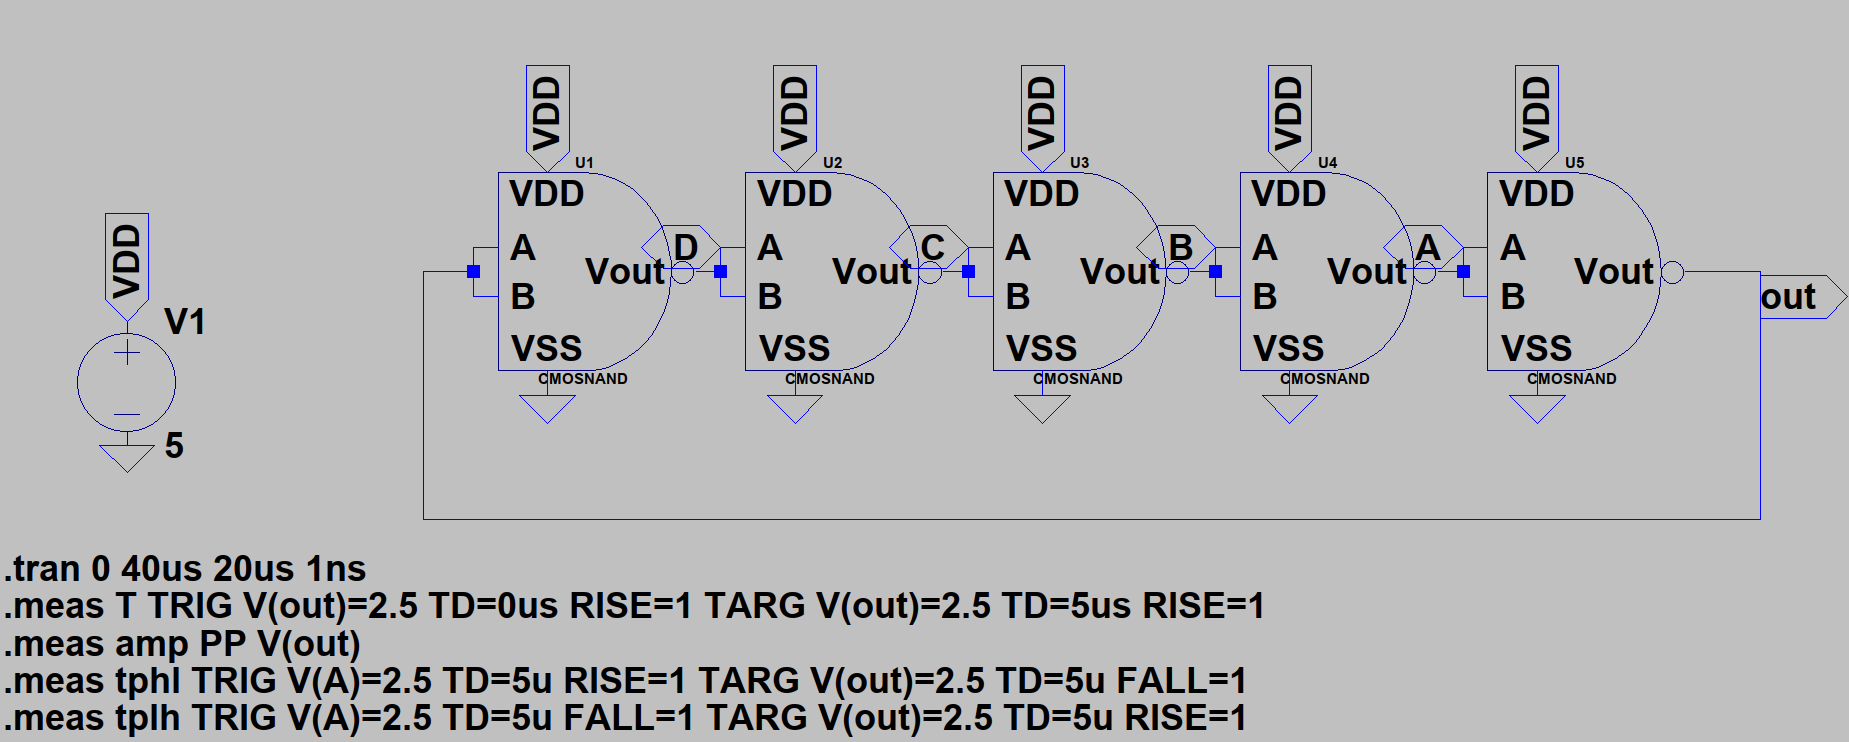
\includegraphics[width=0.6\textwidth]{figures/part_23_circuit.png}
        \caption{The CMOS ring oscillator circuit built in LTspice.}
        \label{fig:ring_circuit}
    \end{figure}
    The circuit above then generates the periodic response shown in
    figure \ref{fig:ring}. Note that the graph is from $20\mu s$ to
    $40\mu s$. The first 20$\mu$s are ignored as the start up is not the
    oscillation motion we are looking for.
    \begin{figure}[H]
        \centering
        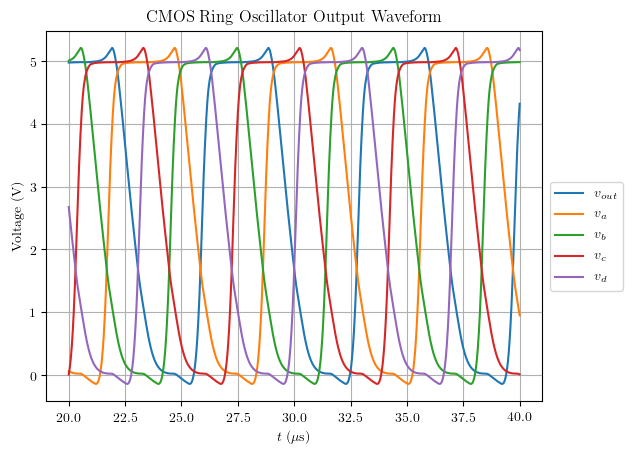
\includegraphics[width=\textwidth]{figures/part_23.png}
        \caption{The oscillation of the CMOS ring oscillator circuit.}
        \label{fig:ring}
    \end{figure}
    The measure statements in the LTspice simulation measure the
    critical values which are shown in table \ref{tab:ring}.
    \begin{table}[H]
        \centering
        \caption{The Measured Values of the CMOS Ring Oscillator.}
        \label{tab:ring}
        \begin{tabular}{c|c}
            &Value\\
            \hline
            $t_s$ & 692.928 ns\\
            $f$ & 144.311 kHz\\
            $A$ & 4.90 V\\
            $T$ & 6.929 $\mu$s\\
        \end{tabular}
    \end{table}
    \subsubsection{Analysis of CMOS Ring Oscillator}
    For the CMOS ring oscillator we find an average propagation delay
    for the NAND gate of 693 ns compared to the 11.2 $\mu$s of the NAND
    gate with common inputs from section \ref{sec:NAND_time}. The reason
    the NAND gates in the ring oscillator have such a significantly
    lower propagation delay is due to fan out. We know that
    \begin{equation}
        t_s = Nt_{s0}\left(1 +
        \frac{\sqrt[N]{\frac{C_L}{C_{g,1}}}}{\gamma}\right)
    \end{equation}
    Assuming that $C_L$ and $C_{g,1}$ are constant between both cases,
    that $\gamma=1$
    and that the input capacitance is around $20pF$
    \footnote{Based on the gate capacitance from the CD4007 LTspice
    component.}
    then $t_s$ will be
    approximately $25t_{s0}$ for the ring oscillator but is almost
    $500t_{s0}$ for the stand alone NAND gate. As such we expect that the
    $t_s$ will be much smaller for the ring oscillator then the NAND
    gate on its own which is what we see.

    Looking at figure \ref{fig:ring} we can see that when 1 signal has
    finished rising the next signal in the chain begins to fall and that
    this occurs $N$ times in 1 period where $N$ is the number of
    inverters in the ring. From this we can see that,
    \begin{equation}
        T = N (t_{PLH} + t_{PHL})
    \end{equation}
    However we can use the fact that $t_s$ is the average of $t_{PLH}$
    and $t_{PHL}$ to write this as
    \begin{equation}\label{eq:ring}
        T = 2Nt_s
    \end{equation}
    Using our measured propagation delay and equation \eqref{eq:ring} we
    would find our period to be 6.93 $\mu$s which is what we measured,
    experimentally verifying our result.


    \pagebreak
    \appendix
    \section*{Appendices}
    \section{Python Code for Data Analysis}\label{sec:code}
    \pythonexternal{lab3.py}
\end{document}
